\begin{figure}
  %\centering
  	\begin{subfigure}{0.45\textwidth}
    \begin{center}
    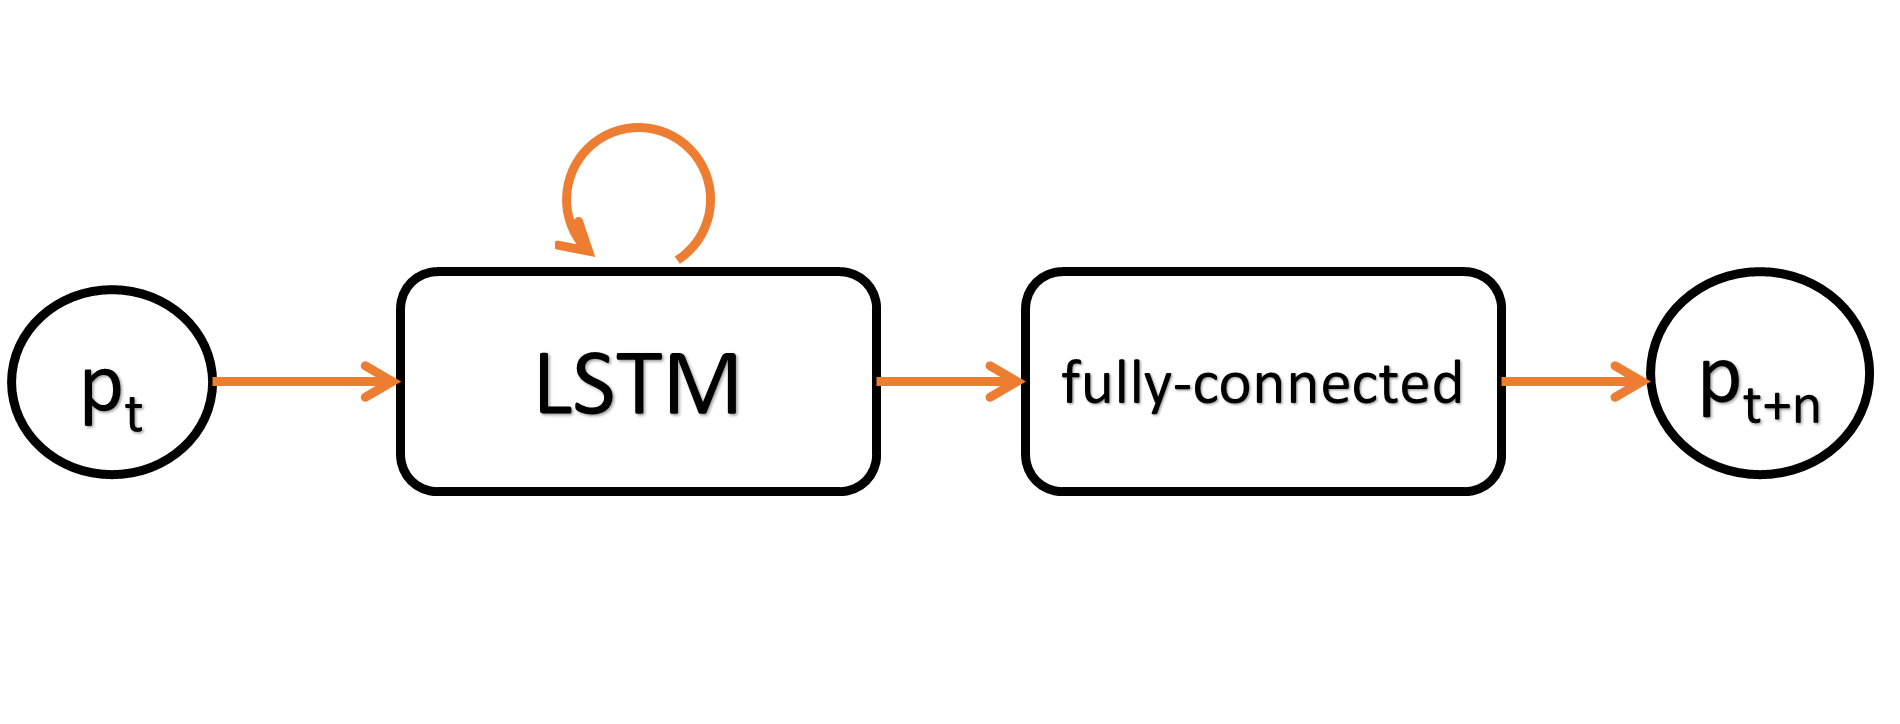
\includegraphics[width=1\textwidth]{img/simple-model.png}
    \end{center}
     \caption{\textbf{Simple model} with the price at the time step \textit{t} as input, and the predicted price at the $n^{th}$ next time step as output}
     \label{simple-model}
  	\end{subfigure}
    \begin{subfigure}{0.45\textwidth}
    \begin{center}
    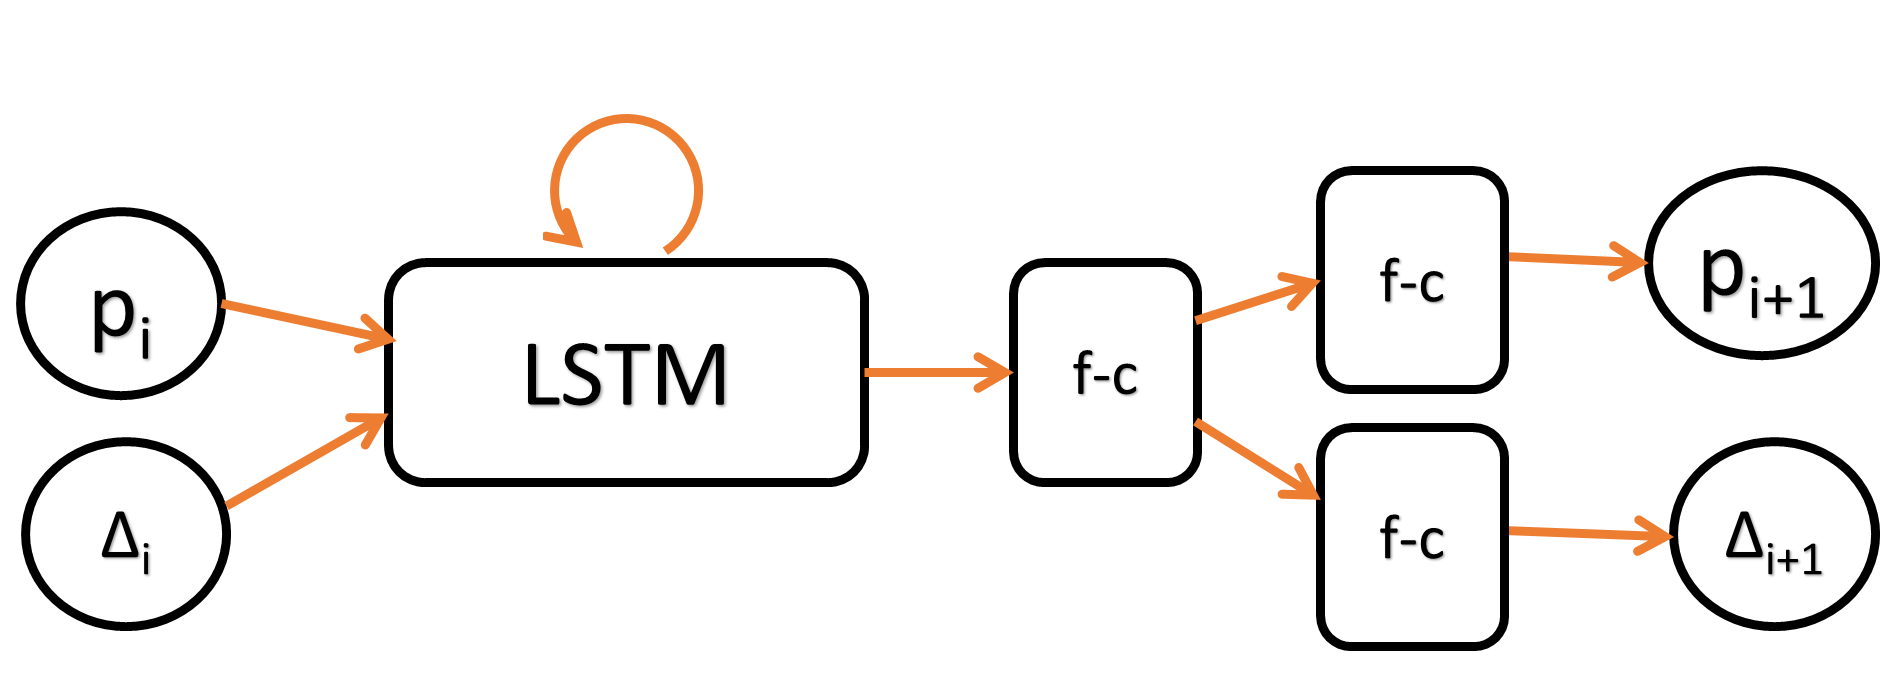
\includegraphics[width=1\textwidth]{img/change-model.png}
    \end{center}
     \caption{\textbf{Change point model} with the price change event as input and the predicted next event as output (both made up of the price update $p_i$ and the time $\delta$ to the last event)}
     \label{change-model}
  	\end{subfigure}
    \caption{The two neural neural network architectures we used to predict the gas price}
\end{figure}